\newcommand{\waves}[5][purple]{
\def\a{1+#3}
\def\b{#3}
\def\c{1-#3}
\def\x{#4}
\def\y{#5}
\foreach \val in {0,#3,...,#2}{
\def\i{\x+\val*4}
\def\var{\y+\val}
\draw[ultra thick, #1] (\i + \b*5,-1+\var) cos (\i + \b*4,0+\var); 
\draw[ultra thick, #1] (\i + \b*4,0+\var) sin (\i + \b*3,\a+\var); 
\draw[ultra thick, #1] (\i + \b*3,\a+\var) cos (\i + \b*2,\b+\var); 
\draw[ultra thick, #1] (\i + \b*2,\b+\var) sin (\i + \b,-\c+\var);}
}
\begin{figure}[h!]
\begin{center}
\scalebox{0.6}{
\begin{tikzpicture}
\waves[green]{1}{0.3}{-6}{3}
\waves[blue]{1}{0.2}{-4}{2}
\waves{1}{0.05}{-2}{1}
\waves{1}{0.05}{0}{0}
\waves[blue]{1}{0.2}{2}{-1}
\waves[green]{1}{0.3}{4}{-2}
\draw(-7, 1.5)--(4,-4);
\draw(4,-4)--(10,-2.5);

\node[right] at (4.5,-5){
\includegraphics[height=35mm]{./Figuras/noise}};
\node[right] at (-10,-3.5){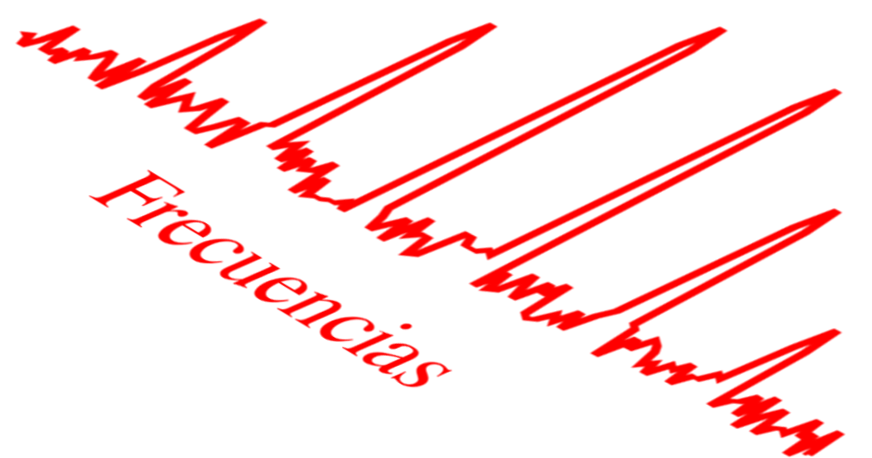
\includegraphics[height=50mm]{./Figuras/freq}};

\end{tikzpicture}}
\end{center}
\caption[Transformada de Fourier]{Comparaci\'on entre una se\~nal y sus frecuencias separadas en ondas individuales.}
\label{fig:trans}
\end{figure}